\chapter{Linear time-invariant systems and convolution}

\section{Example: square wave sent through capacitive cable}
\subsection{A mysterious corruption}
Suppose your friend sitting across the lab\footnote{If you're reading this after 2020, ``labs'' are large classrooms where each desk has its own set of electrical instruments. Usually you work together in teams of 2--3 to build a demo that gets checked off at the end of a 2-hour class.}
badly needs a square wave voltage but doesn't have the equipment to generate one.
Luckily, you do, and you hand over two very long wires plugged into your square wave voltage source.
You're surprised to see a crazy waveform on their oscilloscope.
\begin{center}
  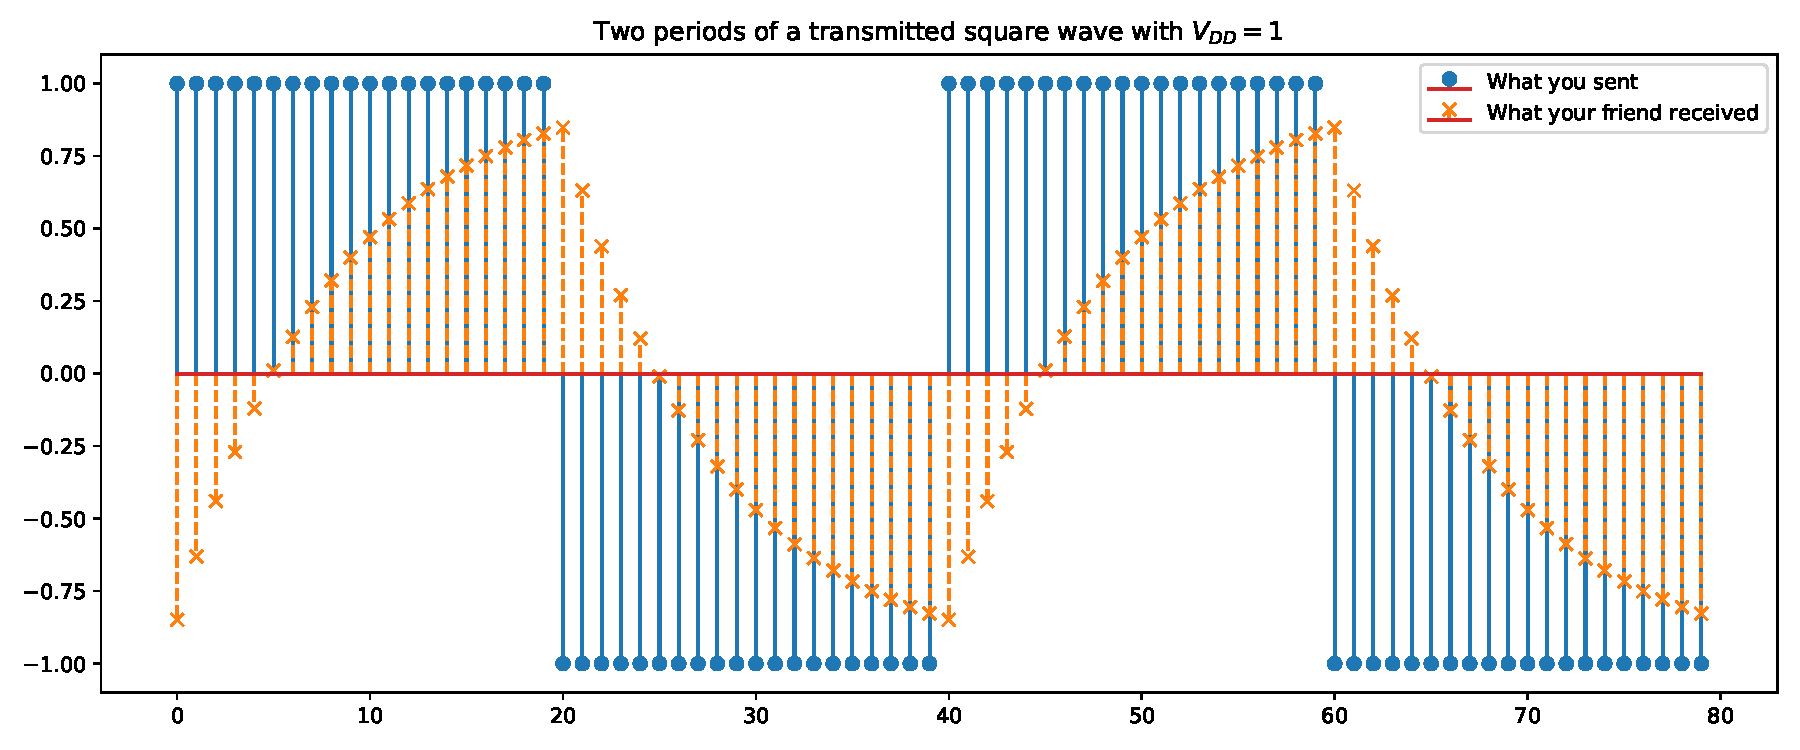
\includegraphics[width=\linewidth]{27-figs/sqwave-lowpassed}
\end{center}
What happened?
The issue is that each wire has a little bit of parasitic resistance \(R\), and there's a parasitic capacitance \(C\) between the two wires.\footnote{Especially if they stay close together.}
The time constant is \(\tau = \frac{1}{2RC}\).

\subsection{Periodic modeling}
We will express a discrete-time model at sampling interval \(T > 0\).
Let \(y[n]\) be the voltage difference at the far end of the cable at time step \(n\), and \(x[n]\) be the voltage difference at the near end.
Then the following recurrence relationship holds:
\begin{align}
  y[n+1]
  &= e^{-T/\tau} y[n] + \del{1 -e^{-T/\tau}} x[n]
  \intertext{Let's choose an even number \(N = M/2\) and send the following square wave:}
  x[n]
  &= \begin{cases}
    1, & n = 0, \ldots, M-1 \quad (\text{mod}\ N)\\
    -1, & n = M, \ldots, N-1 \quad (\text{mod}\ N)
\end{cases}
  \intertext{Therefore we use the state equation to write the following equations describing \(y[1]\) through \(y[N]\):}
  y[1] &= e^{-T/\tau} y[0] + \del{1 - e^{-T/\tau}} x[0] \notag \\
  y[2] &= e^{-T/\tau} y[1] + \del{1 - e^{-T/\tau}} x[1] \notag \\
  \vdots\phantom{[1]} &= \phantom{e^{-T\tau}} \vdots \notag \\
  y[N] &= e^{-T/\tau} y[N - 1] + \del{1 - e^{-T/\tau}} x[N - 1] \notag
  \intertext{Since \(x\) is \(N\)-periodic, so is \(y\) in steady state, so
  \(y[N] = y[0]\) and our last equation is replaced with the following.}
  y[0] &= e^{-T/\tau} y[N - 1] + \del{1 - e^{-T/\tau}} x[N - 1]
  \intertext{
  We can write all \(N\) scalar equations as a single vector equation.
  Treat \(x\) and \(y\) as sample vectors in \(\mathbb{C}^N\).
  Define a circular shift matrix \(S\) such that \((Sy)[n] = y[n+1]\).
  }
  Sy &= e^{-T/\tau} y + \del{1 - e^{-T/\tau}} x \\
  \del{S - e^{-T/\tau} I}y &= \del{1 - e^{-T/\tau}} x \\
  \intertext{We will see later that \(S\)'s eigenvalues are the \(N\)th roots of unity, so \(\del{S - e^{-T/\tau} I}\) is invertible.}
  y &= \del{1 - e^{-T/\tau}}\del{S - e^{-T/\tau} I}^{-1} x.
  \intertext{The matrix \(H \in\mathbb{R}^{n\times n}\) converts a full period of \(x[\cdot]\) to a full period of \(y[\cdot]\). On the near end of the cable \(x\) repeats forever, and on the far end \(Hx\) repeats forever. (Notice that it seems to depend only on things intrinsic to the system itself. It works for any \(x\).)}
  H &= \del{1 - e^{-T/\tau}}\del{S - e^{-T/\tau} I}^{-1}
  \intertext{We will now check that \(H\) makes sense in the cases where \(\tau\) is very small and very large. First, as \(\tau \to 0\), then \(e^{-T/\tau} \to 0\), so}
  H_\text{fast} &= \lim_{\tau \to 0} \del{1 - e^{-T/\tau}}\del{S - e^{-T/\tau} I}^{-1} = S^{-1},
  \intertext{that is, \(y[n] = x[n-1]\). The output waveform is exactly a square wave, reproduced as nearly instantaneously as our sampling interval \(T\) permits. On the other hand}
  H_\text{slow} &=
  \lim_{\tau \to \infty}
  \del{1 - e^{-T/\tau}}\del{S - e^{-T/\tau} I}^{-1} \\
  &= \lim_{\epsilon \to 0} \epsilon \del{S - (1 - \epsilon) I}^{-1}
\end{align}
which is an indeterminate ``0/0'' quotient (numerator becomes zero, and the denominator becomes singular) that I can't find an elementary way to evaluate.\footnote{Let me know if you find one.}

\subsection{In the standard basis}
Let's examine \(H\) by viewing its columns, viz.~the images of the standard basis under \(H\).
Column 0 (the first column) looks like this:
\begin{center}
  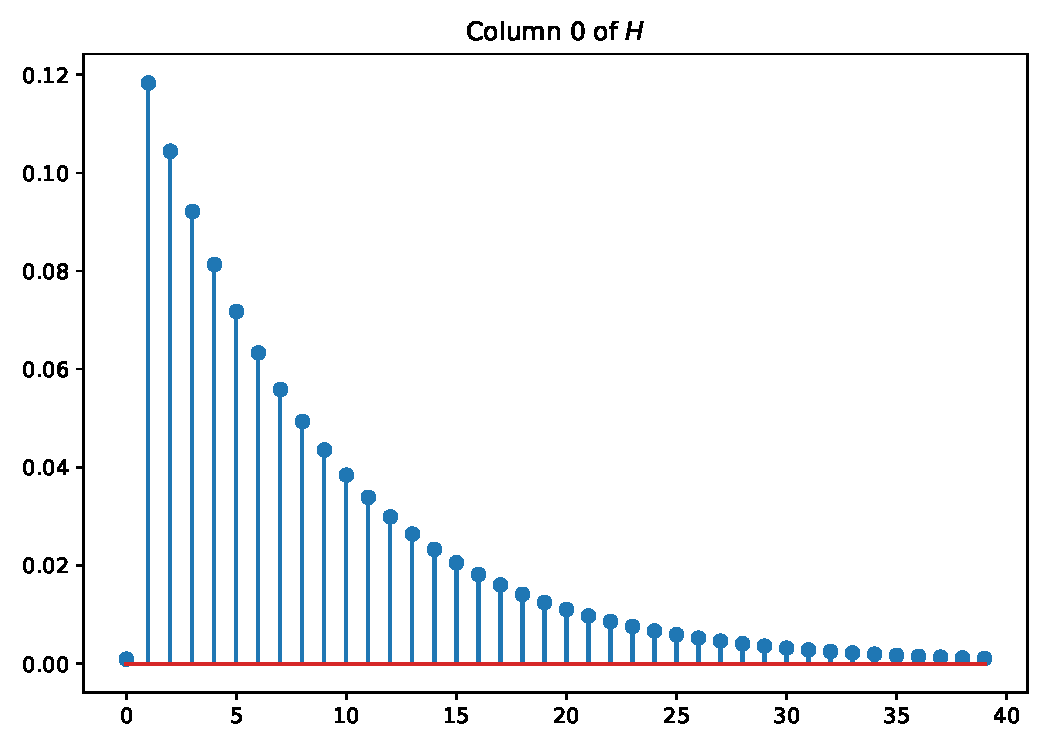
\includegraphics[width=0.618\linewidth]{27-figs/H-0}
\end{center}
and column 1 looks like this:
\begin{center}
  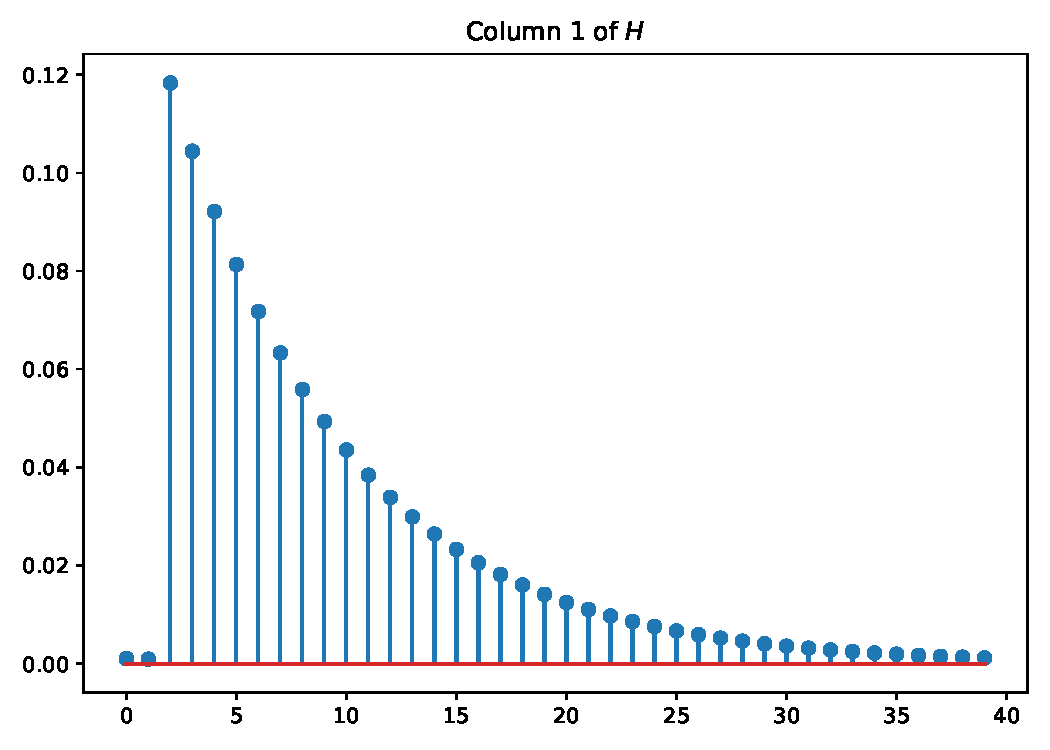
\includegraphics[width=0.618\linewidth]{27-figs/H-1}
\end{center}
You might suspect that column 1 is a right shift\footnote{That is, a right circular shift.} of column 0, and column 2 is a right shift of column 1, and so on.
That would be correct.
% We can prove it like this.
% Because of the circular symmetry of our periodic steady-state equations,
% a shift in the input corresponds to a shift in the output:
% \begin{align}
%   y &= Hx
%   \implies Sy = HSx.
%   % \intertext{We will examine the rela}
% \end{align}

\section{General discrete periodic LTI systems}
Let \(x\in\mathbb{C}^N\) represent a period of input.
Let \(y \in \mathbb{C}^N\) represent a period of input.
A \textbf{linear system} is the relationship\footnote{Lots of \texttt{textbf} ahead! These are definitions!}
\begin{align}
  y &= H x, \quad H \in \mathbb{C}^{N\times N}.
  \intertext{As above, let \(S\) represent a left shift by one sample: \((Sy)[n] = y[n+1]\). If shifts in input correspond to shifts in output, viz.}
  SH &= HS,
  \intertext{the system \(y = Hx\) is called \textbf{time-invariant}.
  Most of our systems from now on with be both linear and time-invariant.
  }
  \intertext{
  When representing periodic signals it is customary to write the standard basis 0-indexed as using the symbol \(\delta_k\) (instead of the ordinary 1-indexed \(e_k\)).}
  \delta_k[n] &=
  \begin{cases}
    1, & n = k\\
    0, & n \neq k
  \end{cases}
  \intertext{\(\delta_i\) is called an \textbf{impulse at time \(i\)}.
  Sometimes \(\delta_0\) is referred to as ``the'' impulse.
  All impulse signals are iterated shifts of \(\delta_0\):}
  \delta_i &= S^{-i} \delta_0
  \intertext{The 0th column of \(H\) is called the \textbf{impulse response} of the linear time-invariant system \(y = Hx\), and it is usually called \(h\).}
  h &= H \delta_0
\end{align}
\section{Convolution: LTI, one impulse at a time}
It is possible to express the LTI system \(y = Hx\) in terms of \(h=H\delta_0\).
Represent \(x\) as a linear combination of standard basis vectors:
\begin{align}
  y &= Hx\\
  &= H\sum_{k = 0}^{N - 1} x[k] \delta_k
  \intertext{Represent each constituent impulse as a shifted \(\delta_0\).}
  &= H\sum_{k = 0}^{N - 1} x[k] \del{S^{-k} \delta_0}\\
  % \intertext{Distribute \(H\) from the left.}
  &= \sum_{k = 0}^{N - 1} x[k] H \del{S^{-k} \delta_0}
  = \sum_{k = 0}^{N - 1} x[k] \del{H S^{-k}} \delta_0
  \intertext{Time-invariance means that \(H\) and \(S\) commute.}
  &= \sum_{k = 0}^{N - 1} x[k] \del{S^{-k} H} \delta_0
  = \sum_{k = 0}^{N - 1} x[k] S^{-k} \del{H\delta_0}\\
  &= \sum_{k = 0}^{N - 1} x[k] S^{-k} h
  \intertext{When \(x = \delta_n\), this equation verifies our earlier observation that all columns of \(H\) are right circular shifts of \(h\). Now let's make a formula for sample \(n\) of the output.}
  y[n] &= \sum_{k = 0}^{N - 1} x[k] \del{S^{-k} h}[n] \\
  &= \sum_{k = 0}^{N - 1} x[k] h[n -k]
  % \intertext{}
\end{align}
This formula is called the \textbf{circular convolution} of \(x\) with \(h\).
